% ============================================================
%  eMeter AMU — User Manual
%  Aligarh Muslim University Electricity Management System
%  Author: Project Documentation
%  Date:   2026
% ============================================================

\documentclass[12pt, a4paper]{report}

% ─── Packages ──────────────────────────────────────────────
\usepackage[utf8]{inputenc}
\usepackage[T1]{fontenc}
\usepackage{geometry}
\usepackage{graphicx}
\usepackage{xcolor}
\usepackage{hyperref}
\usepackage{titlesec}
\usepackage{fancyhdr}
\usepackage{booktabs}
\usepackage{longtable}
\usepackage{array}
\usepackage{enumitem}
\usepackage{listings}
\usepackage{tcolorbox}
\usepackage{fontawesome5}
\usepackage{amsmath}
\usepackage{tabularx}
\usepackage{multirow}
\usepackage{float}
\usepackage{mdframed}
\usepackage{lmodern}
\usepackage{microtype}
\usepackage{parskip}
\usepackage{caption}
\usepackage{subcaption}
\usepackage{tikz}
\usetikzlibrary{shapes.geometric, arrows.meta, positioning, fit, backgrounds, shadows}

% ─── Page Geometry ─────────────────────────────────────────
\geometry{
    left=2.5cm, right=2.5cm,
    top=3cm, bottom=3cm,
    headheight=15pt
}

% ─── Colour Palette ────────────────────────────────────────
\definecolor{primaryGreen}{HTML}{1D9E75}
\definecolor{darkGreen}{HTML}{155E47}
\definecolor{lightGreen}{HTML}{D1FAE5}
\definecolor{accentAmber}{HTML}{F59E0B}
\definecolor{deepBlue}{HTML}{1E3A5F}
\definecolor{lightBlue}{HTML}{DBEAFE}
\definecolor{codeGray}{HTML}{F3F4F6}
\definecolor{textDark}{HTML}{111827}
\definecolor{textMid}{HTML}{374151}
\definecolor{borderColor}{HTML}{E5E7EB}
\definecolor{dangerRed}{HTML}{EF4444}
\definecolor{warningBg}{HTML}{FEF3C7}

% ─── Hyperref Setup ────────────────────────────────────────
\hypersetup{
    colorlinks=true,
    linkcolor=primaryGreen,
    urlcolor=deepBlue,
    citecolor=primaryGreen,
    pdfauthor={eMeter AMU Project},
    pdftitle={eMeter AMU — User Manual},
    pdfsubject={Electricity Billing Management System},
}

% ─── Section Formatting ────────────────────────────────────
\titleformat{\chapter}[display]
    {\normalfont\huge\bfseries\color{deepBlue}}
    {\chaptertitlename\ \thechapter}{20pt}{\Huge\color{primaryGreen}}

\titleformat{\section}
    {\normalfont\Large\bfseries\color{deepBlue}}
    {\thesection}{1em}{}[{\titlerule[1.5pt]}]

\titleformat{\subsection}
    {\normalfont\large\bfseries\color{textMid}}
    {\thesubsection}{1em}{}

\titleformat{\subsubsection}
    {\normalfont\normalsize\bfseries\color{primaryGreen}}
    {\thesubsubsection}{1em}{}

% ─── Header / Footer ───────────────────────────────────────
\pagestyle{fancy}
\fancyhf{}
\fancyhead[L]{\small\textcolor{primaryGreen}{\textbf{eMeter AMU}}}
\fancyhead[R]{\small\textcolor{textMid}{\leftmark}}
\fancyfoot[C]{\small\textcolor{textMid}{\thepage}}
\renewcommand{\headrulewidth}{0.4pt}
\renewcommand{\footrulewidth}{0.4pt}

% ─── Custom Boxes ──────────────────────────────────────────
\tcbuselibrary{skins, breakable, listings}

\newtcolorbox{notebox}[1][]{
    colback=lightBlue, colframe=deepBlue,
    fonttitle=\bfseries,
    title={\faInfoCircle\ \ Note},
    #1
}

\newtcolorbox{warningbox}[1][]{
    colback=warningBg, colframe=accentAmber,
    fonttitle=\bfseries,
    title={\faExclamationTriangle\ \ Warning},
    #1
}

\newtcolorbox{tipbox}[1][]{
    colback=lightGreen, colframe=primaryGreen,
    fonttitle=\bfseries,
    title={\faLightbulb\ \ Tip / Best Practice},
    #1
}

\newtcolorbox{uibox}[2][]{
    colback=codeGray, colframe=borderColor,
    fonttitle=\bfseries\color{deepBlue}\small,
    title={#2},
    #1
}

% ─── Custom env for feature list ───────────────────────────
\newenvironment{featurelist}{%
    \begin{itemize}[leftmargin=1.5em, itemsep=2pt, parsep=0pt]
}{%
    \end{itemize}
}

% ============================================================
\begin{document}

% ─── Cover Page ─────────────────────────────────────────────
\begin{titlepage}
    \centering
    \vspace*{2cm}
    
    % Title Block
    \begin{tcolorbox}[
        colback=deepBlue, colframe=primaryGreen,
        width=\textwidth, arc=8pt, boxrule=2pt
    ]
        \centering
        \vspace{0.5cm}
        {\Huge\bfseries\color{primaryGreen} eMeter AMU}\\[0.4cm]
        {\Large\color{white} Electricity Billing Management System}\\[0.3cm]
        {\large\color{lightGreen} Aligarh Muslim University}\\[0.2cm]
        {\normalsize\color{borderColor} Official User Manual}
        \vspace{0.5cm}
    \end{tcolorbox}
    
    \vspace{1.5cm}
    
    {\large\bfseries\color{textMid} Prepared For:}\\[0.4cm]
    \begin{tabular}{c c c}
        \colorbox{primaryGreen!15}{\textcolor{darkGreen}{\textbf{\ Field Meter Readers\ }}}
        &
        \colorbox{deepBlue!10}{\textcolor{deepBlue}{\textbf{\ Billing Administrators\ }}}
        &
        \colorbox{accentAmber!20}{\textcolor{accentAmber!80!black}{\textbf{\ Consumers\ }}}
    \end{tabular}
    
    \vfill
    
    {\small\color{textMid}
        Version: 1.0\\
        System: eMeter (Django REST Framework + React 18 + React Native)\\[0.3cm]
        \textcolor{borderColor}{\rule{6cm}{0.4pt}}\\[0.3cm]
        \textit{This manual provides detailed instructions on how to use\\
        the eMeter AMU system across Web, Mobile, and Consumer Portals.}
    }
\end{titlepage}

% ─── Table of Contents ──────────────────────────────────────
\tableofcontents

\newpage

% ============================================================
\chapter{System Overview}
% ============================================================

\textbf{eMeter AMU} is a three-tier, cross-platform electricity billing and meter management platform. It digitizes the complete utility billing lifecycle from field meter reading to PDF bill delivery.

\section{System Architecture}

\begin{figure}[H]
\centering
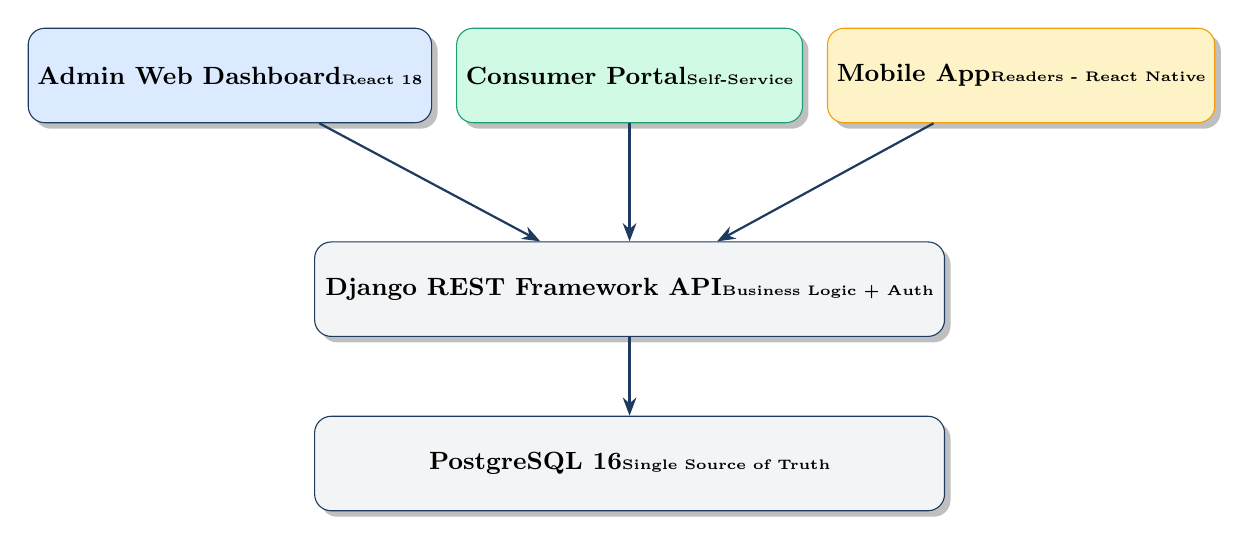
\begin{tikzpicture}[
    node distance=1.5cm,
    box/.style={rectangle, rounded corners=6pt, minimum width=3.5cm, minimum height=1.2cm,
                text centered, font=\small\bfseries, drop shadow},
    arrow/.style={-Stealth, thick, color=deepBlue},
]

% Backend
\node[box, fill=codeGray, draw=deepBlue, minimum width=8cm] (backend) {Django REST Framework API\\{\tiny Business Logic + Auth}};

% Interfaces
\node[box, fill=lightBlue, draw=deepBlue, above left=1.5cm and -1.5cm of backend] (web) {Admin Web Dashboard\\{\tiny React 18}};
\node[box, fill=lightGreen, draw=primaryGreen, above=1.5cm of backend] (portal) {Consumer Portal\\{\tiny Self-Service}};
\node[box, fill=warningBg, draw=accentAmber, above right=1.5cm and -1.5cm of backend] (mobile) {Mobile App\\{\tiny Readers - React Native}};

% Database
\node[box, fill=codeGray, draw=deepBlue, below=1cm of backend, minimum width=8cm] (db) {PostgreSQL 16\\{\tiny Single Source of Truth}};

% Arrows
\draw[arrow] (web) -- (backend);
\draw[arrow] (portal) -- (backend);
\draw[arrow] (mobile) -- (backend);
\draw[arrow] (backend) -- (db);

\end{tikzpicture}
\caption{eMeter System Ecosystem}
\end{figure}

\section{User Roles}

\begin{table}[H]
\centering
\begin{tabularx}{\textwidth}{>{\bfseries}l l X}
\toprule
Role & Interface & Access Level \\
\midrule
Administrator & Web Dashboard & Full system control, billing configuration, consumer management, and reports. \\
Meter Reader & Mobile App + Web & Submit readings, view assigned history, perform offline sync. \\
Consumer & Consumer Portal & Read-only access to own bills and readings, download PDFs. \\
\bottomrule
\end{tabularx}
\end{table}

% ============================================================
\chapter{Admin Web Dashboard}
% ============================================================

The Admin Web Dashboard is accessed via a web browser. Administrators and meter readers with web access use this interface.

\section{Logging In}

\textbf{URL:} \texttt{http://your-server-address} (or the deployed domain)

\begin{enumerate}
    \item Open the web dashboard URL in your browser (Chrome, Firefox, or Safari recommended).
    \item You will be taken to the Login Page.
    \item Enter your Username and Password provided by the system administrator.
    \item Click \textbf{Sign In}.
\end{enumerate}

\begin{notebox}
If you see a "Session Expired" error, your security token has timed out. Simply log in again to continue working.
\end{notebox}

\section{Dashboard Overview}

After login, you land on the Dashboard Overview — a real-time snapshot of the entire system.

\textbf{Summary Cards (click any to navigate):}
\begin{itemize}[leftmargin=1.5em]
    \item \textbf{Total Consumers:} Number of registered electricity connections
    \item \textbf{Meter Readings:} Total reading records submitted to the system
    \item \textbf{Revenue (Paid):} Total collections (sum of paid bills in Rs.)
    \item \textbf{Pending Amount:} Outstanding unpaid bill total in Rs.
    \item \textbf{Current Consumption:} kWh billed in the current month
    \item \textbf{Total Bills:} Total number of invoices generated
\end{itemize}

\textbf{Quick Action Buttons (top right):}
\begin{itemize}[leftmargin=1.5em]
    \item \textbf{Add Consumer} opens the Add Consumer form
    \item \textbf{New Reading} (Reader role only) opens the Reading submission form
    \item \textbf{Billing} navigates to the Billing module
\end{itemize}

\section{Managing Consumers}

\textbf{Navigate:} Sidebar $\rightarrow$ Consumers

This page lists all registered consumers with their meter numbers, status, and account type.

\subsection{Adding a New Consumer}
\begin{enumerate}
    \item Click \textbf{+ Add Consumer} (top right).
    \item Fill in the form. Required fields include \textbf{Full Name} and \textbf{Meter Number}. Optional fields include Consumer ID (auto-generated if left blank), Phone, Address, Post, Department, Initial Reading, Load (KW), Account Type, Phase, and Status.
    \item Click \textbf{Save Consumer}.
\end{enumerate}

\subsection{Editing and Viewing Consumer Details}
\begin{enumerate}
    \item Find the consumer in the list using the global search bar.
    \item Click the three-dot (\textit{more}) menu in the Actions column.
    \item Select \textbf{Edit} to modify details or \textbf{View} to open a detail panel showing all connection metrics.
\end{enumerate}
\textit{Note: The Initial Reading field is hidden during editing to prevent accidental modification of historical data.}

\subsection{Resetting a Consumer's Portal Password}
If a consumer forgets their self-service portal password:
\begin{enumerate}
    \item Click the three-dot menu $\rightarrow$ \textbf{Reset Portal Password}.
    \item Confirm the action.
    \item The consumer's portal password is reset to their Consumer Number (e.g., \texttt{CN001234}). Inform the consumer to log in and immediately change their password.
\end{enumerate}

\section{Meter Readings Module}

\textbf{Navigate:} Sidebar $\rightarrow$ Readings

This module is the central hub for recording and tracking electricity consumption.

\subsection{Viewing Reading History for a Consumer}
\begin{enumerate}
    \item Find the consumer in the table.
    \item Click the \textbf{History (clock icon)} button on the right.
    \item A history modal opens with a complete chronological table of all readings.
\end{enumerate}
From the History Modal, you can filter by date, print the report, or export it to Excel.

\subsection{Submitting a New Reading (Meter Reader Role)}
\textit{This feature is visible only to users with the Reader role via the web panel.}
\begin{enumerate}
    \item Click \textbf{+ New Reading}.
    \item Select the consumer from the dropdown. The Previous Reading auto-fills.
    \item Enter the Current Reading in kWh. The Units Consumed is calculated live.
    \item Click \textbf{Save Reading}.
\end{enumerate}

\subsection{Administrative Bill Entry (Admin Only)}
Administrators can manually create a bill for a consumer (e.g., for paper-based readings):
\begin{enumerate}
    \item Click \textbf{Generate Bills $\rightarrow$ Administrative Bill Entry}.
    \item Select the consumer, enter the Current Reading, set the Billing Month, Due Date, and an optional manual override reason.
    \item Click \textbf{Submit Administrative Entry}.
\end{enumerate}

\section{Billing Module}

\textbf{Navigate:} Sidebar $\rightarrow$ Billing

This is the complete billing ledger. Every generated bill is listed here. The top of the page shows cumulative \textbf{Total Billed}, \textbf{Collected}, and \textbf{Pending} amounts.

\subsection{Bill Actions}
Click the three-dot menu next to any bill to access:
\begin{itemize}
    \item \textbf{View Details:} Opens a modal with full charge breakdown.
    \item \textbf{Mark as Paid / Unpaid:} Toggles the payment status.
    \item \textbf{Download PDF:} Generates and downloads a formatted PDF invoice.
    \item \textbf{Print PDF:} Opens a browser print dialog with the formatted bill.
\end{itemize}

\subsection{Exporting and Printing Bills}
Click \textbf{Download Excel} to download all currently filtered bills as a structured \texttt{.xlsx} file. Click \textbf{Print Report} to print a hardcopy summary.

\section{Import Readings via Excel (Admin Only)}

\textbf{Navigate:} Sidebar $\rightarrow$ Import Readings

This feature allows administrators to upload a batch of meter readings from an Excel file to generate bills in bulk.

\subsection{Upload Process}
\begin{enumerate}
    \item Click \textbf{Download Template} to get a pre-formatted \texttt{.xlsx} file.
    \item Fill the template (do not delete the header row).
    \item Drag and drop your \texttt{.xlsx} file onto the upload zone.
    \item Click \textbf{Import \& Generate Bills}.
\end{enumerate}

\begin{tipbox}
\textbf{Accepted Excel Formats:}\\
\textbf{4-Column (Recommended):} Consumer Number | Meter Number | Current Reading | Reading Date\\
\textbf{3-Column (Legacy):} Consumer Number | Current Reading | Reading Date\\
\textit{Date format must be YYYY-MM-DD or DD-MM-YYYY. Blank dates default to today.}
\end{tipbox}

\section{Reports Module}

\textbf{Navigate:} Sidebar $\rightarrow$ Reports

The Reports page shows live, visual analytics pulled directly from the database:
\begin{itemize}
    \item \textbf{Monthly Usage Trends (Bar Chart):} Shows consumption trends over the past months.
    \item \textbf{Revenue Breakdown (Donut Chart):} Split between Paid and Unpaid revenue.
    \item \textbf{Top 10 Consumers (Progress Bars):} Lists the highest-consuming connections.
\end{itemize}

\section{Settings and Billing Configuration (Admin Only)}

\textbf{Navigate:} Sidebar $\rightarrow$ Settings

\subsection{Billing Configuration (Tariff Engine)}
This is the dynamic tariff engine. Changes here affect all future bill calculations.

\begin{table}[H]
\centering
\begin{tabularx}{\textwidth}{>{\bfseries}l X}
\toprule
Setting & Description \\
\midrule
Default Unit Rate & Price per kWh consumed (e.g., Rs. 8.56) \\
Default Tax / Duty & Electricity duty percentage applied on energy charges (e.g., 7.5\%) \\
Fixed Charge per kW & Monthly fixed connection charge per KW of load (e.g., Rs. 400) \\
Phase Meter Rents & Monthly rent based on connection type (1-Phase / 3-Phase) \\
\bottomrule
\end{tabularx}
\end{table}

\begin{warningbox}
Rate changes only affect \textbf{new} bills generated after the update. All past bills are permanently locked to the rates that were active at the time they were created.
\end{warningbox}

\subsection{Mobile App Sync Offline Sync File}
When meter readers operate in offline mode without internet, they can still use pre-loaded consumer data. Click \textbf{Export Sync File} to download \texttt{eMeter\_Offline\_Sync.json}. Share this file with the meter reader to import into their mobile app.

% ============================================================
\chapter{Consumer Self-Service Portal}
% ============================================================

The Consumer Portal is a separate, read-only interface where individual consumers can view their own billing information securely.

\section{Consumer Login}
\textbf{URL:} \texttt{http://your-server-address/consumer/login}

\begin{enumerate}
    \item Enter your \textbf{Consumer Number} (e.g., \texttt{CN001234}) as the username.
    \item Enter your \textbf{Password} (default is your Consumer Number, unless changed).
    \item Click \textbf{Sign In}.
\end{enumerate}

\section{Consumer Dashboard}
The profile card displays your connection status, registered address, and meter details. A statistics grid summarizes your total bills, paid bills, and unpaid bills. 

\section{Viewing My Readings}
\textbf{Navigate:} Consumer Dashboard $\rightarrow$ My Readings\\
Displays a chronological table of every meter reading recorded for your connection, including the date, previous reading, current reading, and total units consumed.

\section{Viewing and Downloading My Bills}
\textbf{Navigate:} Consumer Dashboard $\rightarrow$ My Bills\\
Lists all your generated bills. To download a bill:
\begin{enumerate}
    \item Find the bill row you require.
    \item Click the \textbf{Download PDF} (or Print) icon.
    \item A formatted electricity invoice opens with full charge breakdown and payment status watermark.
\end{enumerate}

\section{Changing Password}
\textbf{Navigate:} Consumer Dashboard $\rightarrow$ Change Password\\
Enter your current password, and your new password twice. 
\textit{Use a password at least 8 characters long with a mix of letters and numbers.}

% ============================================================
\chapter{Mobile App Meter Reader Guide}
% ============================================================

The eMeter Mobile App is designed for field meter readers. It supports both \textbf{online} and \textbf{offline} operation.

\section{Installation and Login}
Install the app on your Android (8.0+) or iOS (13+) smartphone. Open the app, enter your assigned Username and Password, and tap \textbf{Sign In}.

\section{Mobile Dashboard}
The dashboard adapts based on network availability:
\begin{itemize}
    \item \textbf{Status Badge:} Shows a green dot (Online) or yellow dot (Offline).
    \item \textbf{Daily Sync Tracker:} Shows progress towards your daily reading target.
    \item \textbf{Offline Queue Alert:} A yellow banner appears when readings are saved locally but not yet synced to the server.
\end{itemize}

\section{Setting Up Consumer Data (Online or Offline)}

\subsection{Pull Registry (Online)}
Before going into the field while connected to internet:
\begin{enumerate}
    \item Tap \textbf{Pull Registry} on the Dashboard.
    \item The app downloads the latest consumer list and tariff settings to your phone.
\end{enumerate}
\textit{Best Practice: Pull the registry every morning before going into the field.}

\subsection{Import Data (Total Offline)}
If you have no internet but received a sync file from the administrator:
\begin{enumerate}
    \item Tap \textbf{Import Data} on the Dashboard.
    \item Select the \texttt{eMeter\_Offline\_Sync.json} file.
    \item The app will load all consumer data entirely offline.
\end{enumerate}

\section{Submitting a Meter Reading}

\begin{enumerate}
    \item Tap \textbf{Search and Submit}.
    \item Type the consumer's name or meter number. Tap their card.
    \item Verify the Previous Reading shown.
    \item Enter the \textbf{Current Reading} shown on the physical meter. (Must be greater than or equal to the previous reading).
    \item As you type, the app calculates a \textbf{Live Bill Estimate}.
    \item Tap \textbf{Submit and Generate Bill}.
\end{enumerate}

\begin{notebox}
\textbf{What happens next:}\\
The reading is always saved locally first. If internet is available, the bill is generated immediately and a preview is shown. If offline, the app alerts you that the reading is saved locally and will sync later.
\end{notebox}

\section{Offline Syncing and Queue Management}

When your phone reconnects to the internet, tap \textbf{Sync} on the yellow dashboard banner to push all queued readings to the server. Bills are generated automatically.

\textbf{Offline Queue Inspector:}\\
Tap the offline banner to view all pending readings. If a sync fails, the error message (e.g., duplicate reading) will be displayed here. You can optionally delete an incorrect pending reading from this inspector.

\textbf{Export to Excel:}\\
Tap \textbf{Excel} on the offline queue banner to generate an \texttt{.xlsx} file of your pending readings to manually share with the billing office via WhatsApp or email.

% ============================================================
\chapter{Appendix}
% ============================================================

\section{Role Permission Reference}

\begin{table}[H]
\centering
\begin{tabularx}{\textwidth}{X c c c}
\toprule
\textbf{Feature} & \textbf{Admin} & \textbf{Meter Reader} & \textbf{Consumer} \\
\midrule
View Dashboard & Yes & Yes & Yes (own) \\
Add/Edit/Delete Consumers & Yes & No & No \\
Submit Readings (Web) & No & Yes & No \\
Submit Readings (App) & Yes & Yes & No \\
Administrative Bill Entry & Yes & No & No \\
Import Excel (Bulk) & Yes & No & No \\
View All Bills & Yes & Yes & No \\
View Own Bills & No & No & Yes \\
Mark Bill Paid/Unpaid & Yes & No & No \\
Download PDF Bills & Yes & Yes (after submit) & Yes \\
View Reports & Yes & No & No \\
Edit Billing Settings & Yes & No & No \\
\bottomrule
\end{tabularx}
\end{table}

\section{Billing Calculation Formula}

\begin{uibox}{The billing calculation is automatic. Here is how the total is computed:}
\begin{verbatim}
1. Units Consumed  = Current Reading - Previous Reading
2. Energy Charges  = Units Consumed x Rate per Unit (Rs./kWh)
3. Fixed Charges   = Load (KW) x Fixed Charge per KW
4. Duty Charge     = (Energy Charges + Fixed Charges) x Duty % / 100
5. Meter Rent      = Phase-1 Rent (Single Phase) or Phase-3 Rent
6. Regulatory Surcharge = (as configured)
7. Arrears         = Outstanding amount from previous unpaid bill
8. Late Surcharge  = Applied if payment is past due date

Grand Total = Sum of items 2 through 8
\end{verbatim}
\end{uibox}

\section{Common Troubleshooting}

\begin{table}[H]
\centering
\begin{tabularx}{\textwidth}{>{\bfseries}l X X}
\toprule
Problem & Likely Cause & Solution \\
\midrule
Session Expired & JWT token timed out & Log in again \\
Cannot delete consumer & Consumer has existing bills & Mark consumer as Inactive instead \\
Reading rejected & Current < Previous & Re-check the physical meter and enter the correct value \\
Import Excel error & Duplicate reading & Only one reading per consumer per billing month is allowed \\
Sync fails for consumer & Duplicate / Server error & Check error log in Queue Inspector \\
Bill shows Rs.0 & Billing settings were zero & Admin must update Billing Configuration in Settings \\
\bottomrule
\end{tabularx}
\end{table}

\vspace{2em}
\hrule
\vspace{1em}

\begin{center}
\textit{Document generated for eMeter AMU — Electricity Billing and Meter Management System}\\[0.2cm]
\textit{Aligarh Muslim University, Department of Computer Science}\\[0.2cm]
{\small For technical issues, contact the system administrator.}
\end{center}

\end{document}
